% Created 2018-12-12 Wed 15:41
% Intended LaTeX compiler: pdflatex
\documentclass[11pt]{article}
\usepackage[utf8]{inputenc}
\usepackage[T1]{fontenc}
\usepackage{graphicx}
\usepackage{grffile}
\usepackage{longtable}
\usepackage{wrapfig}
\usepackage{rotating}
\usepackage[normalem]{ulem}
\usepackage{amsmath}
\usepackage{textcomp}
\usepackage{amssymb}
\usepackage{capt-of}
\usepackage{hyperref}
\usepackage{minted}
\author{Anoop G R}
\date{\today}
\title{}
\hypersetup{
 pdfauthor={Anoop G R},
 pdftitle={},
 pdfkeywords={},
 pdfsubject={},
 pdfcreator={Emacs 26.1 (Org mode 9.1.9)}, 
 pdflang={English}}
\begin{document}

\tableofcontents

\section{Top Index}
\label{sec:orge92e371}

Foundations

$$ How Do I Get Started?
$$ Step-by-Step Process
$$ Linear Algebra
$$ Statistical Methods

Beginner

$$ Understand Algorithms
$$ Weka ML (no code)
$$ Python ML (scikit-learn)
$$ R ML (caret)

Intermediate

$$ Code Algorithms (Python)
$$ Time Series Forecasting
$$ XGBoost Algorithm
$$ Deep Learning (Keras)

Advanced

$$ Deep Learning and LSTMs
$$ Deep Learning for Text
\$\$ Deep Learning for Time Series Forecasting


\section{Anoop index:}
\label{sec:org7cb2e88}
How Do I Get Started?
Applied Machine Learning Process
Linear Algebra
Statistical Methods
Understand Machine Learning Algorithms
Python Machine Learning (scikit-learn)
Code Algorithm from Scratch (Python)
Introduction to Time Series Forecasting (Python)
XGBoost in Python (Stochastic Gradient Boosting)
Deep Learning (Keras)
Long Short-Term Memory (LSTM)
Deep Learning for Natural Language Processing (NLP)
Deep Learning for Time Series Forecasting

\section{(edited to top anoop, rest of page) Applied Machine Learning Process}
\label{sec:orgfcd3a32}

The benefit of machine learning are the predictions and the models that make predictions.

To have skill at applied machine learning means knowing how to consistently and reliably deliver high-quality predictions on problem after problem. You need to follow a systematic process.

Below is a 5-step process that you can follow to consistently achieve above average results on predictive modeling problems:

\$\$ Step 1: Define your problem. 

\$\$ How to Define Your Machine Learning Problem

\$\$ Step 2: Prepare your data. 

$$ How to Prepare Data For Machine Learning
 $$ How to Identify Outliers in your Data
$$ Improve Model Accuracy with Data Pre-Processing
 $$ Discover Feature Engineering
$$ An Introduction to Feature Selection
 $$ Tactics to Combat Imbalanced Classes in Your Machine Learning Dataset
\$\$ Data Leakage in Machine Learning

\$\$ Step 3: Spot-check algorithms. 

$$ How to Evaluate Machine Learning Algorithms
 $$ Why you should be Spot-Checking Algorithms on your Machine Learning Problems
$$ How To Choose The Right Test Options When Evaluating Machine Learning Algorithms
 $$ A Data-Driven Approach to Choosing Machine Learning Algorithms

\$\$ Step 4: Improve results. 

$$ How to Improve Machine Learning Results
 $$ Machine Learning Performance Improvement Cheat Sheet
\$\$ How To Improve Deep Learning Performance

\$\$ Step 5: Present results. 

$$ How to Use Machine Learning Results
 $$ How to Train a Final Machine Learning Model
\$\$ How To Deploy Your Predictive Model To Production

For a good summary of this process, see the posts:

$$ Applied Machine Learning Process
$$ How to Use a Machine Learning Checklist to Get Accurate Predictions

Linear Algebra

Linear algebra is an important foundation area of mathematics required for achieving a deeper understanding of machine learning algorithms.

Below is the 3 step process that you can use to get up-to-speed with linear algebra for machine learning, fast.

\$\$ Step 1: Discover what Linear Algebra is. 

\$\$ A Gentle Introduction to Linear Algebra

\$\$ Step 2: Discover why Linear Algebra is important for machine learning. 

$$ 5 Reasons to Learn Linear Algebra for Machine Learning
 $$ Linear Algebra for Machine Learning

\$\$ Step 3: Dive into Linear Algebra topics. 

$$ Linear Algebra for Machine Learning Mini-Course
 $$ Linear Algebra for Machine Learning (my book)

You can see all linear algebra posts here. Below is a selection of some of the most popular tutorials.

Linear Algebra in Python

$$ Introduction to N-Dimensional Arrays in Python
$$ How to Index, Slice and Reshape NumPy Arrays

Matrices

$$ Introduction to Matrices and Matrix Arithmetic
$$ Introduction to Matrix Types in Linear Algebra

Vectors

$$ Introduction to Vectors
$$ Introduction to Vector Norms

Matrix Factorization

$$ Introduction to Matrix Factorization
$$ Introduction to Eigendecomposition

Statistical Methods

Statistical Methods an important foundation area of mathematics required for achieving a deeper understanding of the behavior of machine learning algorithms.

Below is the 3 step process that you can use to get up-to-speed with statistical methods for machine learning, fast.

\$\$ Step 1: Discover what Statistical Methods are. 

\$\$ What is Statistics (and why is it important in machine learning)?

\$\$ Step 2: Discover why Statistical Methods are important for machine learning. 

$$  The Close Relationship Between Applied Statistics and Machine Learning
 $$  10 Examples of How to Use Statistical Methods in a Machine Learning Project

\$\$ Step 3: Dive into the topics of Statistical Methods. 

$$ Statistics for Machine Learning (7-Day Mini-Course)
 $$ Statistical Methods for Machine Learning (my book)

You can see all of the statistical methods posts here. Below is a selection of some of the most popular tutorials.

Summary Statistics

$$ Introduction to the 5 Number Summary
$$ Introduction to Data Visualization

Hypothesis Tests

$$ 15 Hypothesis Tests (cheat sheet)
$$ Tests for Comparing Algorithms

Resampling Methods

$$ Introduction to the Bootstrap
$$ Introduction to Cross-Validation

Estimation Statistics

$$ Introduction to Estimation Statistics
$$ Introduction to Confidence Intervals

Understand Machine Learning Algorithms

Machine learning is about machine learning algorithms.

You need to know what algorithms are available for a given problem, how they work, and how to get the most out of them.

Here’s how to get started with machine learning algorithms:

\$\$ Step 1: Discover the different types of machine learning algorithms. 

\$\$ A Tour of Machine Learning Algorithms

\$\$ Step 2: Discover the foundations of machine learning algorithms. 

$$ How Machine Learning Algorithms Work
 $$ Parametric and Nonparametric Algorithms
$$ Supervised and Unsupervised Algorithms
 $$ The Bias-Variance Trade-Off
\$\$ Overfitting and Underfitting With Algorithms

\$\$ Step 3: Discover how top machine learning algorithms work. 

$$ Machine Learning Algorithms Mini-Course
 $$ Master Machine Learning Algorithms (my book)

You can see all machine learning algorithm posts here. Below is a selection of some of the most popular tutorials.

Linear Algorithms

$$ Gradient Descent
$$ Linear Regression
$$ Logistic Regression
$$ Linear Discriminant Analysis

Nonlinear Algorithms

$$ Classification And Regression Trees
$$ Naive Bayes
$$ K-Nearest Neighbors
$$ Learning Vector Quantization
\$\$ Support Vector Machines

Ensemble Algorithms

$$ Bagging and Random Forest
$$ Boosting and AdaBoost

Weka Machine Learning (no code)

Weka is a platform that you can use to get started in applied machine learning.

It has a graphical user interface meaning that no programming is required and it offers a suite of state of the art algorithms.

Here’s how you can get started with Weka:

\$\$ Step 1: Discover the features of the Weka platform. 

\$\$ What is the Weka Machine Learning Workbench

\$\$ Step 2: Discover how to get around the Weka platform. 

$$ How to Download and Install the Weka Machine Learning Workbench
 $$ A Tour of the Weka Machine Learning Workbench

\$\$ Step 3: Discover how to deliver results with Weka. 

$$ How to Run Your First Classifier in Weka
 $$ Applied Machine Learning With Weka Mini-Course
\$\$ Machine Learning Mastery With Weka (my book)

You can see all Weka machine learning posts here. Below is a selection of some of the most popular tutorials.

Prepare Data in Weka

$$ How To Load CSV Machine Learning Data in Weka
$$ How to Better Understand Your Machine Learning Data in Weka
$$ How to Normalize and Standardize Your Machine Learning Data in Weka
$$ How To Handle Missing Values In Machine Learning Data With Weka
\$\$ How to Perform Feature Selection With Machine Learning Data in Weka

Weka Algorithm Tutorials

$$ How to Use Machine Learning Algorithms in Weka
$$ How To Estimate The Performance of Machine Learning Algorithms in Weka
$$ How To Use Regression Machine Learning Algorithms in Weka
$$ How To Use Classification Machine Learning Algorithms in Weka
\$\$ How to Tune Machine Learning Algorithms in Weka

Python Machine Learning (scikit-learn)

Python is one of the fastest growing platforms for applied machine learning.

You can use the same tools like pandas and scikit-learn in the development and operational deployment of your model.

Below are the steps that you can use to get started with Python machine learning:

\$\$ Step 1: Discover Python for machine learning 

\$\$ A Gentle Introduction to Scikit-Learn: A Python Machine Learning Library

\$\$ Step 2: Discover the ecosystem for Python machine learning. 

$$ Crash Course in Python for Machine Learning Developers
 $$ Python Ecosystem for Machine Learning
\$\$ Python is the Growing Platform for Applied Machine Learning

\$\$ Step 3: Discover how to work through problems using machine learning in Python. 

$$ Your First Machine Learning Project in Python Step-By-Step
 $$ Python Machine Learning Mini-Course
\$\$ Machine Learning Mastery With Python (my book)

You can see all Python machine learning posts here. Below is a selection of some of the most popular tutorials.

Prepare Data in Python

$$ How To Load Machine Learning Data in Python
$$ Understand Your Machine Learning Data With Descriptive Statistics in Python
$$ Visualize Machine Learning Data in Python With Pandas
$$ How To Prepare Your Data For Machine Learning in Python with Scikit-Learn
\$\$ Feature Selection For Machine Learning in Python

Machine Learning in Python

$$ Evaluate the Performance of Machine Learning Algorithms
$$ Metrics To Evaluate Machine Learning Algorithms in Python
$$ Spot-Check Classification Machine Learning Algorithms in Python with scikit-learn
$$ Spot-Check Regression Machine Learning Algorithms in Python with scikit-learn
\$\$ How To Compare Machine Learning Algorithms in Python with scikit-learn

R Machine Learning (caret)

R is a platform for statistical computing and is the most popular platform among professional data scientists.

It’s popular because of the large number of techniques available, and because of excellent interfaces to these methods such as the powerful caret package.

Here’s how to get started with R machine learning:

\$\$ Step 1: Discover the R platform and why it is so popular. 

$$ What is R
 $$ Use R For Machine Learning
\$\$ Super Fast Crash Course in R

\$\$ Step 2: Discover machine learning algorithms in R. 

\$\$ How To Get Started With Machine Learning Algorithms in R

\$\$ Step 3: Discover how to work through problems using machine learning in R. 

$$ Your First Machine Learning Project in R Step-By-Step
 $$ R Machine Learning Mini-Course
\$\$ Machine Learning Mastery With R (my book)

You can see all R machine learning posts here. Below is a selection of some of the most popular tutorials.

Data Preparation in R

$$ How To Load Your Machine Learning Data Into R
$$ Better Understand Your Data in R Using Descriptive Statistics
$$ Better Understand Your Data in R Using Visualization
$$ Feature Selection with the Caret R Package
\$\$ Get Your Data Ready For Machine Learning in R with Pre-Processing

Applied Machine Learning in R

$$ How to Evaluate Machine Learning Algorithms with R
$$ Spot Check Machine Learning Algorithms in R
$$ Tune Machine Learning Algorithms in R
$$ How to Build an Ensemble Of Machine Learning Algorithms in R
\$\$ Compare The Performance of Machine Learning Algorithms in R

Code Algorithm from Scratch (Python)

You can learn a lot about machine learning algorithms by coding them from scratch.

Learning via coding is the preferred learning style for many developers and engineers.

Here’s how to get started with machine learning by coding everything from scratch.

\$\$ Step 1: Discover the benefits of coding algorithms from scratch. 

$$ Benefits of Implementing Machine Learning Algorithms From Scratch
 $$ Understand Machine Learning Algorithms By Implementing Them From Scratch

\$\$ Step 2: Discover that coding algorithms from scratch is a learning tool only. 

\$\$ Stop Coding Machine Learning Algorithms From Scratch

\$\$ Step 3: Discover how to code machine learning algorithms from scratch in Python. 

\$\$ Machine Learning Algorithms From Scratch (my book)

You can see all of the Code Algorithms from Scratch posts here. Below is a selection of some of the most popular tutorials.

Prepare Data

$$ How to Load Machine Learning Data From Scratch
$$ How to Scale Machine Learning Data From Scratch

Linear Algorithms

$$ How To Implement Simple Linear Regression From Scratch
$$ How To Implement The Perceptron Algorithm From Scratch

Algorithm Evaluation

$$ How to Code Resampling Methods From Scratch
$$ How To Code Algorithm Performance Metrics From Scratch

Nonlinear Algorithms

$$ How to Code the Backpropagation Algorithm From Scratch
$$ How To Code The Decision Tree Algorithm From Scratch

Introduction to Time Series Forecasting (Python)

Time series forecasting is an important topic in business applications.

Many datasets contain a time component, but the topic of time series is rarely covered in much depth from a machine learning perspective.

Here’s how to get started with Time Series Forecasting:

\$\$ Step 1: Discover Time Series Forecasting. 

\$\$ What Is Time Series Forecasting?

\$\$ Step 2: Discover Time Series as Supervised Learning. 

\$\$ Time Series Forecasting as Supervised Learning

\$\$ Step 3: Discover how to get good at delivering results with Time Series Forecasting. 

$$ Time Series Forecasting With Python Mini-Course
 $$ Time Series Forecasting With Python (my book)

You can see all Time Series Forecasting posts here. Below is a selection of some of the most popular tutorials.

Data Preparation Tutorials

$$ 7 Time Series Datasets for Machine Learning
$$ How to Load and Explore Time Series Data in Python
$$ How to Normalize and Standardize Time Series Data in Python
$$ Basic Feature Engineering With Time Series Data in Python
\$\$ How To Backtest Machine Learning Models for Time Series Forecasting

Forecasting Tutorials

$$ How to Make Baseline Predictions for Time Series Forecasting with Python
$$ How to Check if Time Series Data is Stationary with Python
$$ How to Create an ARIMA Model for Time Series Forecasting with Python
$$ How to Grid Search ARIMA Model Hyperparameters with Python
\$\$ How to Work Through a Time Series Forecast Project

XGBoost in Python (Stochastic Gradient Boosting)

XGBoost is a highly optimized implementation of gradient boosted decision trees.

It is popular because it is being used by some of the best data scientists in the world to win machine learning competitions.

Here’s how to get started with XGBoost:

\$\$ Step 1: Discover the Gradient Boosting Algorithm. 

\$\$ A Gentle Introduction to the Gradient Boosting Algorithm for Machine Learning

\$\$ Step 2: Discover XGBoost. 

\$\$ A Gentle Introduction to XGBoost for Applied Machine Learning

\$\$ Step 3: Discover how to get good at delivering results with XGBoost. 

$$ How to Develop Your First XGBoost Model in Python with scikit-learn
 $$ XGBoost With Python Mini-Course
\$\$ XGBoost With Python (my book)

You can see all XGBoosts posts here. Below is a selection of some of the most popular tutorials.

XGBoost Basics

$$ Data Preparation for Gradient Boosting with XGBoost in Python
$$ How to Evaluate Gradient Boosting Models with XGBoost in Python
$$ Avoid Overfitting By Early Stopping With XGBoost In Python
$$ Feature Importance and Feature Selection With XGBoost in Python

XGBoost Tuning

$$ How to Configure the Gradient Boosting Algorithm
$$ Tune Learning Rate for Gradient Boosting with XGBoost in Python
$$ Stochastic Gradient Boosting with XGBoost and scikit-learn in Python
$$ How to Tune the Number and Size of Decision Trees with XGBoost in Python
\$\$ How to Best Tune Multithreading Support for XGBoost in Python

Deep Learning (Keras)

Deep learning is a fascinating and powerful field.

State-of-the-art results are coming from the field of deep learning and it is a sub-field of machine learning that cannot be ignored.

Here’s how to get started with deep learning:

\$\$ Step 1: Discover what deep learning is all about. 

$$ What is Deep Learning?
 $$ 8 Inspirational Applications of Deep Learning

\$\$ Step 2: Discover the best tools and libraries. 

$$ Introduction to the Python Deep Learning Library Theano
 $$ Introduction to the Python Deep Learning Library TensorFlow
\$\$ Introduction to Python Deep Learning with Keras

\$\$ Step 3: Discover how to work through problems and deliver results. 

$$ Develop Your First Neural Network in Python With Keras Step-By-Step
 $$ Applied Deep Learning in Python Mini-Course
\$\$ Deep Learning With Python (my book)

You can see all deep learning posts here. Below is a selection of some of the most popular tutorials.

Background

$$ Crash Course On Multi-Layer Perceptron Neural Networks
$$ Crash Course in Convolutional Neural Networks for Machine Learning
\$\$ Crash Course in Recurrent Neural Networks for Deep Learning

Multilayer Perceptrons

$$ 5 Step Life-Cycle for Neural Network Models in Keras
$$ How to Grid Search Hyperparameters for Deep Learning Models in Python With Keras
$$ Save and Load Your Keras Deep Learning Models
$$ Display Deep Learning Model Training History in Keras
\$\$ Dropout Regularization in Deep Learning Models With Keras

Convolutional Neural Networks

$$ Handwritten Digit Recognition using Convolutional Neural Networks in Python with Keras
$$ Object Recognition with Convolutional Neural Networks in the Keras Deep Learning Library
\$\$ Predict Sentiment From Movie Reviews Using Deep Learning

Recurrent Neural Networks

$$ Time Series Prediction with LSTM Recurrent Neural Networks in Python with Keras
$$ Understanding Stateful LSTM Recurrent Neural Networks in Python with Keras
\$\$ Text Generation With LSTM Recurrent Neural Networks in Python with Keras

Long Short-Term Memory (LSTM)

Long Short-Term Memory (LSTM) Recurrent Neural Networks are designed for sequence prediction problems and are a state-of-the-art deep learning technique for challenging prediction problems.

Here’s how to get started with LSTMs in Python:

\$\$ Step 1: Discover the promise of LSTMs. 

\$\$ The Promise of Recurrent Neural Networks for Time Series Forecasting

\$\$ Step 2: Discover where LSTMs are useful. 

$$ Making Predictions with Sequences
 $$ A Gentle Introduction to Long Short-Term Memory Networks by the Experts
\$\$ Introduction to Models for Sequence Prediction

\$\$ Step 3: Discover how to use LSTMs on your project. 

$$ The 5 Step Life-Cycle for Long Short-Term Memory Models in Keras
 $$ Long Short-Term Memory Networks (Mini-Course)
\$\$ Long Short-Term Memory Networks With Python (my book)

You can see all LSTM posts here. Below is a selection of some of the most popular tutorials using LSTMs in Python with the Keras deep learning library.

Data Preparation for LSTMs

$$ How to Reshape Input Data for Long Short-Term Memory Networks
$$ How to One Hot Encode Sequence Data
$$ How to Remove Trends and Seasonality with a Difference Transform
$$ How to Scale Data for Long Short-Term Memory Networks
$$ How to Prepare Sequence Prediction for Truncated BPTT
$$ How to Handle Missing Timesteps in Sequence Prediction Problems

LSTM Behaviour

$$ A Gentle Introduction to Backpropagation Through Time
$$ Demonstration of Memory with a Long Short-Term Memory Network
$$ How to Use the TimeDistributed Layer for Long Short-Term Memory Networks
$$ How to use an Encoder-Decoder LSTM to Echo Sequences of Random Integers
\$\$ Attention in Long Short-Term Memory Recurrent Neural Networks

Modeling with LSTMs

$$ Generative Long Short-Term Memory Networks
$$ Stacked Long Short-Term Memory Networks
$$ Encoder-Decoder Long Short-Term Memory Networks
$$ CNN Long Short-Term Memory Networks
$$ Diagnose Overfitting and Underfitting of LSTM Models
$$ How to Make Predictions with Long Short-Term Memory Models

LSTM for Time Series

$$ On the Suitability of LSTMs for Time Series Forecasting
$$ Time Series Forecasting with the Long Short-Term Memory Network
$$ Multi-step Time Series Forecasting with Long Short-Term Memory Networks
$$ Multivariate Time Series Forecasting with LSTMs in Keras

Deep Learning for Natural Language Processing (NLP)

Working with text data is hard because of the messy nature of natural language.

Text is not “solved” but to get state-of-the-art results on challenging NLP problems, you need to adopt deep learning methods

Here’s how to get started with deep learning for natural language processing:

\$\$ Step 1: Discover what deep learning for NLP is all about. 

$$ What is Natural Language Processing?
 $$ What is Deep Learning?
\$\$ Promise of Deep Learning for Natural Language Processing

\$\$ Step 2: Discover standard datasets for NLP. 

$$ 7 Applications of Deep Learning for Natural Language Processing
 $$ Datasets for Natural Language Processing

\$\$ Step 3: Discover how to work through problems and deliver results. 

$$ Crash-Course in Deep Learning for Natural Language Processing
 $$ Deep Learning for Natural Language Processing (my book)

You can see all deep learning for NLP posts here. Below is a selection of some of the most popular tutorials.

Bag-of-Words Model

$$ What is the Bag-of-Words Model?
$$ How to Prepare Text Data for Machine Learning with scikit-learn
\$\$ How to Develop a Bag-of-Words Model for Predicting Sentiment

Language Modeling

$$ Gentle Introduction to Statistical Language Modeling and Neural Language Models
$$ How to Develop a Character-Based Neural Language Model in Keras
\$\$ How to Develop a Word-Level Neural Language Model and Use it to Generate Text

Text Summarization

$$ A Gentle Introduction to Text Summarization
$$ How to Prepare News Articles for Text Summarization
\$\$ Encoder-Decoder Models for Text Summarization in Keras

Word Embeddings

$$ What are Word Embeddings?
$$ How to Develop Word Embeddings in Python with Gensim
\$\$ How to Use Word Embedding Layers for Deep Learning with Keras

Photo Captioning

$$ How to Automatically Generate Textual Descriptions for Photographs with Deep Learning
$$ A Gentle Introduction to Deep Learning Caption Generation Models
\$\$ How to Develop a Deep Learning Photo Caption Generator from Scratch

Text Translation

$$ A Gentle Introduction to Neural Machine Translation
$$ How to Configure an Encoder-Decoder Model for Neural Machine Translation
\$\$ How to Develop a Neural Machine Translation System from Scratch

Deep Learning for Time Series Forecasting

Deep learning neural networks are able to automatically learn arbitrary complex mappings from inputs to outputs and support multiple inputs and outputs.

Methods such as MLPs, CNNs, and LSTMs offer a lot of promise for time series forecasting.

Here’s how to get started with deep learning for time series forecasting:

\$\$ Step 1: Discover the promise (and limitations) of deep learning for time series. 

$$ The Promise of Recurrent Neural Networks for Time Series Forecasting
 $$ On the Suitability of Long Short-Term Memory Networks for Time Series Forecasting
\$\$ Results From Comparing Classical and Machine Learning Methods for Time Series Forecasting

\$\$ Step 2: Discover how to develop robust baseline and defensible forecasting models. 

$$ Taxonomy of Time Series Forecasting Problems
 $$ How to Develop a Skillful Machine Learning Time Series Forecasting Model

\$\$ Step 3: Discover how to build deep learning models for time series forecasting. 

$$ How to Get Started with Deep Learning for Time Series Forecasting (7-Day Mini-Course)
 $$ Deep Learning for Time Series Forecasting (my book)

You can see all deep learning for time series forecasting posts here. Below is a selection of some of the most popular tutorials.

Forecast Trends and Seasonality (univariate)

$$ Grid Search SARIMA Models for Time Series Forecasting
$$ Grid Search Exponential Smoothing for Time Series Forecasting
\$\$ Develop Deep Learning Models for Univariate Forecasting

Human Activity Recognition (multivariate classification)

$$ How to Model Human Activity From Smartphone Data
$$ How to Develop CNN Models for Human Activity Recognition
\$\$ How to Develop RNN Models for Human Activity Recognition

Forecast Electricity Usage (multivariate, multi-step)

$$ How to Load and Explore Household Electricity Usage Data
$$ Multi-step Time Series Forecasting with Machine Learning
\$\$ How to Develop CNNs for Multi-Step Time Series Forecasting

Models Types

$$ How to Develop MLPs for Time Series Forecasting
$$ How to Develop CNNs for Time Series Forecasting
\$\$ How to Develop LSTMs for Time Series Forecasting

Time Series Case Studies

$$ Indoor Movement Time Series Classification
$$ Probabilistic Forecasting Model to Predict Air Pollution Days
$$ Predict Room Occupancy Based on Environmental Factors
$$ Predict Whether Eyes are Open or Closed Using Brain Waves

Forecast Air Pollution (multivariate, multi-step)

$$ Load, Visualize, and Explore a Air Pollution Forecasting
$$ Develop Baseline Forecasts for Air Pollution Forecasting
$$ Develop Autoregressive Models for Air Pollution Forecasting
$$ Develop Machine Learning Models for Air Pollution Forecasting

Need More Help?

I’m here to help you become awesome at applied machine learning.

If you still have questions and need help, you have some options:

\$\$ Ebooks: I sell a catalog of Ebooks that show you how to get results with machine learning, fast. 

\$\$ Machine Learning Mastery EBook Catalog

\$\$ Blog: I write a lot about applied machine learning on the blog, try the search feature. 

\$\$ Machine Learning Mastery Blog

\$\$ Frequently Asked Questions: The most common questions I get and their answers 

\$\$ Machine Learning Mastery FAQ

\$\$ Contact: You can contact me with your question, but one question at a time please. 

\$\$ Machine Learning Mastery Contact

© 2018 Machine Learning Mastery. All Rights Reserved. 



\section{experimental0}
\label{sec:org9e2acc7}
chrome history suggestions based on a neural network
read to get ideas for projects: \url{https://machinelearningmastery.com/self-study-machine-learning-projects/}
maintain a ml daily blog?
how to get computers to talk to each other using socket programming
use free time with phone to study google maps of Bangalore like guttapalli
buy toothbrush, bigger bulb for room
sabji kitne ki hai app

\section{How Do I Get Started?}
\label{sec:org01190d1}

\subsection{articles-read, worth rereading}
\label{sec:orgcd57423}
$$ Applied Machine Learning Process
 $$ Intermediate: Python Ecosystem.

\$\$ Step 4: Practice on Datasets. Select datasets to work on and practice the process. 

$$ Practice Machine Learning with Small In-Memory Datasets
 $$ Tour of Real-World Machine Learning Problems
\$\$ Work on Machine Learning Problems That Matter To You

\$\$ Step 5: Build a Portfolio. Gather results and demonstrate your skills. 

$$ Build a Machine Learning Portfolio
 $$ Get Paid To Apply Machine Learning
\$\$ Machine Learning For Money

For more on this top-down approach, see:

$$ The Machine Learning Mastery Method
$$ Machine Learning for Programmers

Many of my students have used this approach to go on and do well in Kaggle competitions and get jobs as Machine Learning Engineers and Data Scientists.

\subsection{notes}
\label{sec:org9885175}

\subsubsection{intro}
\label{sec:orgce5e49f}
sckit-learn is higher level than numpy \& scipy
machine learning is a subset of artificial intelligence
artificial learning is a more consistent name for machine learning

\subsubsection{some key word definitions:}
\label{sec:org7dc374b}
Model: A machine learning model can be a mathematical representation
of a real-world process. To generate a machine learning model you will
need to provide training data to a machine learning algorithm to learn
from.

Algorithm: Machine Learning algorithm is the hypothesis set that is
taken at the beginning before the training starts with real-world
data. When we say Linear Regression algorithm, it means a set of
functions that define similar characteristics as defined by Linear
Regression and from those set of functions we will choose one function
that fits the most by the training data.

Training: While training for machine learning, you pass an algorithm
with training data. The learning algorithm finds patterns in the
training data such that the input parameters correspond to the target.
The output of the training process is a machine learning model which
you can then use to make predictions. This process is also called
“learning”.

Regression: Regression techniques are used when the output is
real-valued based on continuous variables. For example, any time
series data. This technique involves fitting a line.

Classification: In classification, you will need to categorize data
into predefined classes. For example, an email can either be ‘spam’ or
‘not spam’.

Target: The target is whatever the output of the input variables. It
could be the individual classes that the input variables maybe mapped
to in case of a classification problem or the output value range in a
regression problem. If the training set is considered then the target
is the training output values that will be considered.

Feature: Features are individual independent variables that act as the
input in your system. Prediction models use features to make
predictions. New features can also be obtained from old features using
a method known as ‘feature engineering’. More simply, you can consider
one column of your data set to be one feature. Sometimes these are
also called attributes. And the number of features are called
dimensions.

Label: Labels are the final output. You can also consider the output
classes to be the labels. When data scientists speak of labeled data,
they mean groups of samples that have been tagged to one or more
labels.

Overfitting: An important consideration in machine learning is how
well the approximation of the target function that has been trained
using training data, generalizes to new data. Generalization works
best if the signal or the sample that is used as the training data has
a high signal to noise ratio. If that is not the case, generalization
would be poor and we will not get good predictions. A model is
overfitting if it fits the training data too well and there is a poor
generalization of new data.

Regularization: Regularization is the method to estimate a preferred
complexity of the machine learning model so that the model generalizes
and the over-fit/under-fit problem is avoided. This is done by adding
a penalty on the different parameters of the model thereby reducing
the freedom of the model.

Parameter and Hyper-Parameter: Parameters are configuration variables
that can be thought to be internal to the model as they can be
estimated from the training data. Algorithms have mechanisms to
optimize parameters. On the other hand, hyperparameters cannot be
estimated from the training data. Hyperparameters of a model are set
and tuned depending on a combination of some heuristics and the
experience and domain knowledge of the data scientist.


\section{\url{https://machinelearningmastery.com/python-machine-learning-mini-course/}}
\label{sec:org707410d}
14Lessons
\subsection{pre requisite \url{https://machinelearningmastery.com/gentle-introduction-to-the-bias-variance-trade-off-in-machine-learning/}}
\label{sec:org3af63c3}
\textbf{Bias Error}
Bias are the simplifying assumptions made by a model to make the target function easier to learn.
Low Bias: Suggests less assumptions about the form of the target function.
High-Bias: Suggests more assumptions about the form of the target function.

Examples of low-bias machine learning algorithms include: Decision Trees, k-Nearest Neighbors and Support Vector Machines.
Examples of high-bias machine learning algorithms include: Linear Regression, Linear Discriminant Analysis and Logistic Regression.

\textbf{Variance Error}
Variance is the amount that the estimate of the target function will change if different training data was used.

Examples of low-variance machine learning algorithms include: Linear Regression, Linear Discriminant Analysis and Logistic Regression.
Examples of high-variance machine learning algorithms include: Decision Trees, k-Nearest Neighbors and Support Vector Machines.

Fig 1. bulls-eye visualise \url{http://scott.fortmann-roe.com/docs/BiasVariance.html}

\subsection{1 - install}
\label{sec:org51abaaa}
\subsubsection{next time try using this tutorial \url{https://sourabhbajaj.com/mac-setup/Python/numpy.html}}
\label{sec:org64f8908}
\subsubsection{make a new virtualenv}
\label{sec:orgf4872ae}
\begin{minted}[]{shell}
pwd
\end{minted}


Use :session: property to speed up org-babel when possible to use the same session
\begin{minted}[]{bash}
source ~/.bashrc
#mkvirtualenv mlm
workon mlm
which python
\end{minted}

\begin{minted}[]{elisp}
(pyvenv-workon "mlm2")
\end{minted}

\subsubsection{install \url{https://stackoverflow.com/questions/26319762/how-to-install-scipy-stack-with-pip-and-homebrew}}
\label{sec:org7caeea9}
pip install numpy
brew install gcc
pip install scipy
brew install freetype
pip install matplotlib
pip install nose
pip install pandas
pip install sympy
pip install ipython[all]
brew install pyqt
brew install qt
brew install sip
\#after this edit the 2 scripts
\subsubsection{check if properly isntalled using .\_\(_{\text{version}}\) \_ after import}
\label{sec:org86e42a5}

using python snippets inside orgmode \url{https://orgmode.org/worg/org-contrib/babel/languages/ob-doc-python.html}
installed python-mode from package-list-packages for emacs
\begin{minted}[]{common-lisp}
(pyvenv-workon "mlm")
\end{minted}

Fixed some errors using: pip install nose pyparsing python-dateutil pep8
\begin{minted}[]{python}
import sys
import scipy
import numpy
import matplotlib
import pandas
import sklearn

print(f'python: {sys.version}')
print(f'scipy: {scipy.__version__}')
print(f'numpy: {numpy.__version__}')
print(f'matplotlib {matplotlib.__version__}')
print(f'pandas {pandas.__version__}')
print(f'sklearn {sklearn.__version__}')

\end{minted}

\subsection{2 - python, pandas, numpy, mathplotlib veeery basics}
\label{sec:org8bc6077}

\subsubsection{python, also refer in-y-minutes file for future reference}
\label{sec:org53fa719}
\begin{minted}[]{python}
if 1>2:
    print("wtf")
else:
    print("ok")

try:
    # Use "raise" to raise an error
    raise IndexError("This is an index error")
except IndexError as e:
    print("its indexerror")
    pass                 # Pass is just a no-op. Usually you would do recovery here.
except (TypeError, NameError):
    print("its typeerror or nameerror")
    pass                 # Multiple exceptions can be handled together, if required.
else:                    # Optional clause to the try/except block. Must follow all except blocks
    print("All good!")   # Runs only if the code in try raises no exceptions
finally:                 #  Execute under all circumstances
    print("We can clean up resources here")
\end{minted}

\begin{minted}[]{python}
def accepts_variable_number_of_arguments(*args):
    print(type(args))
    print(args)

accepts_variable_number_of_arguments(1,2,3)

def accepts_variable_number_of_keyword_arguments(**kwargs):
    print(type(kwargs))
    print(kwargs)

accepts_variable_number_of_keyword_arguments(name="anoop", work="code")
\end{minted}

\subsubsection{numpy basics}
\label{sec:orgdd229f4}

\begin{center}
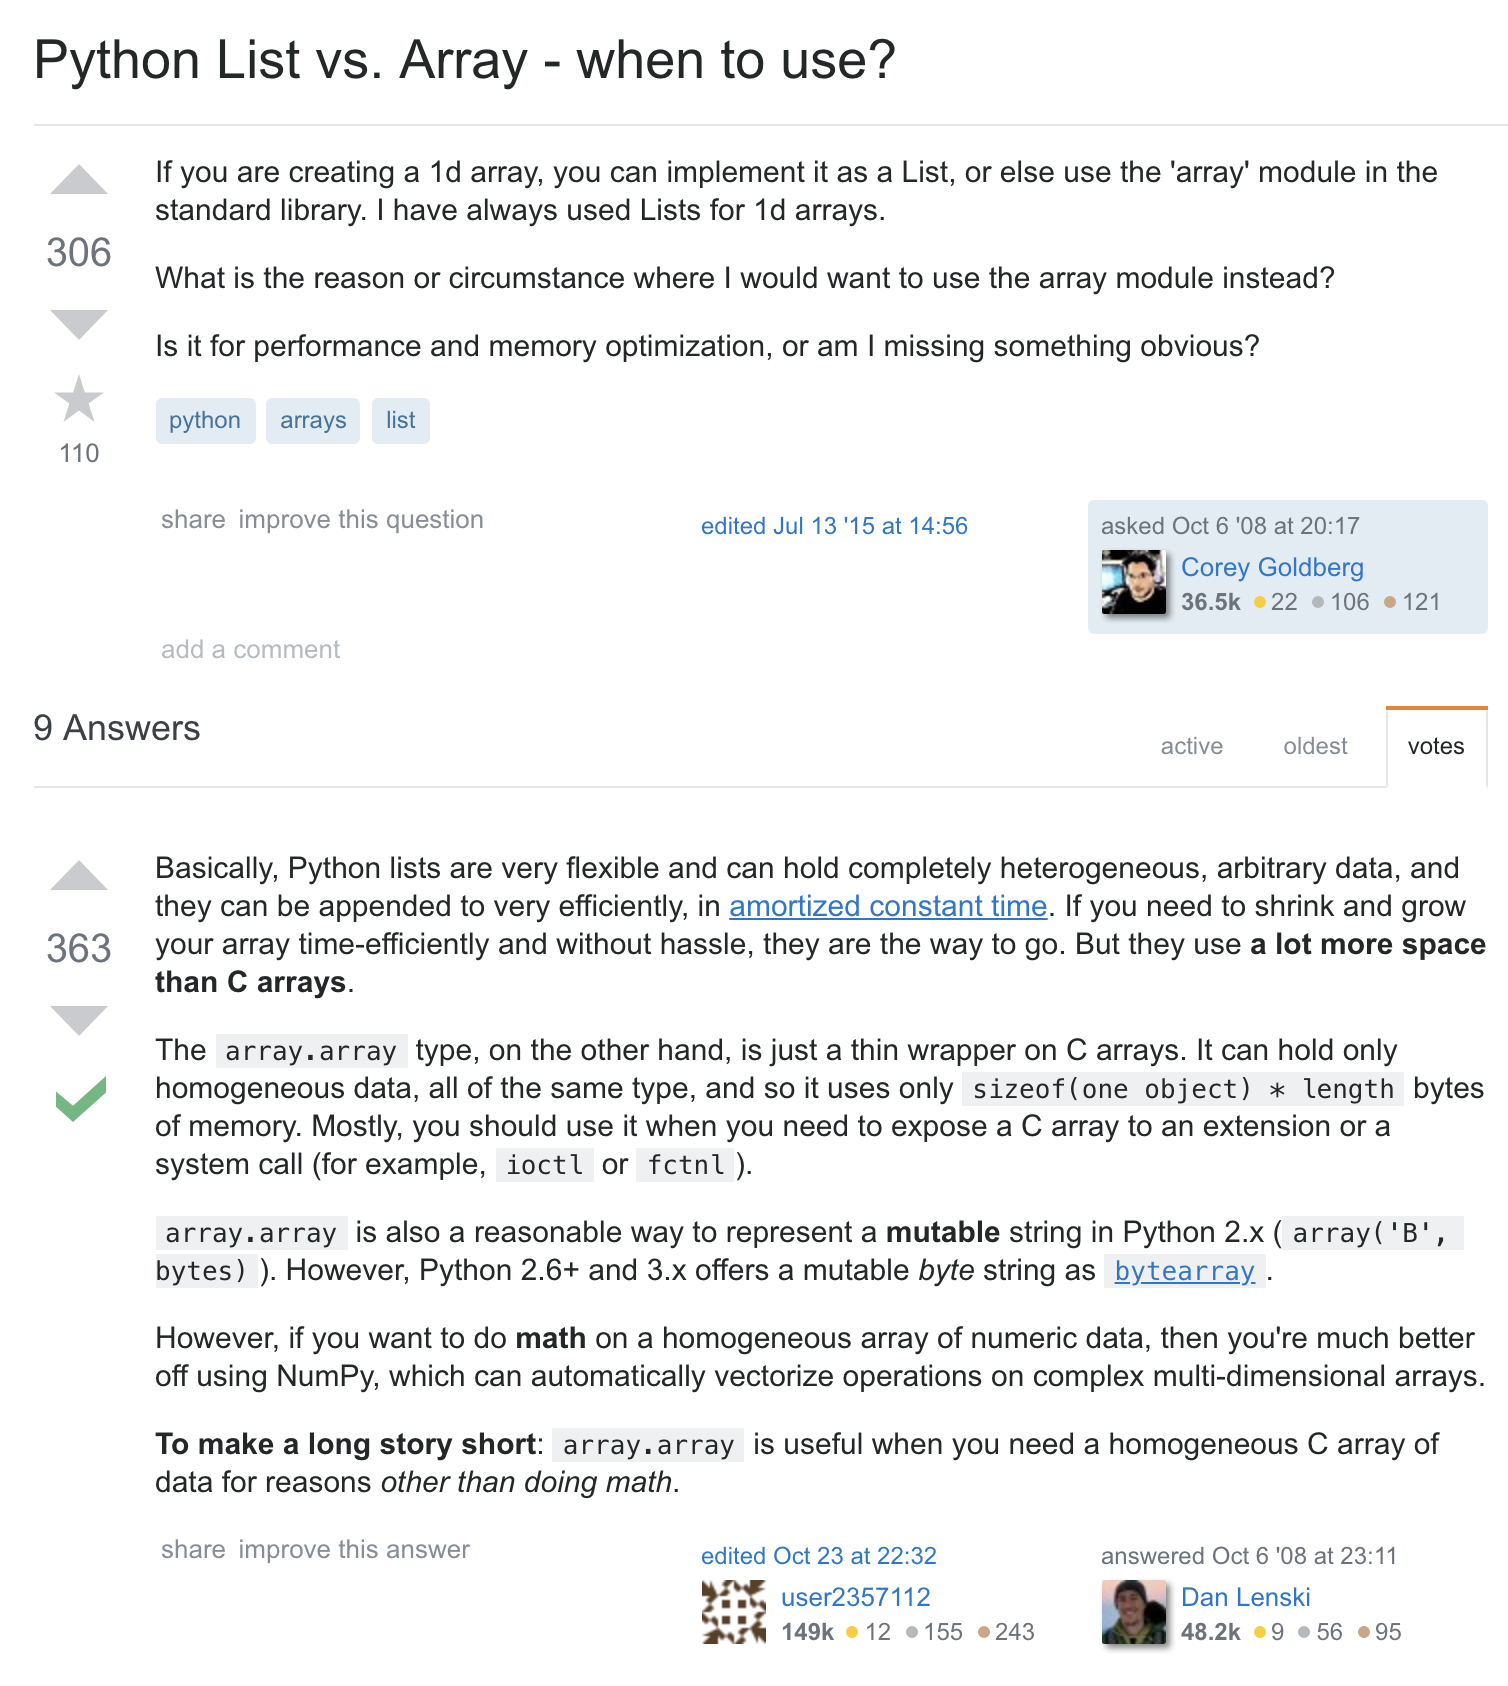
\includegraphics[width=.9\linewidth]{screenshots0/Screenshot 2018-12-11 at 5.16.28 PM.png}
\end{center}

\textbf{numpy official tutorial}
\url{https://docs.scipy.org/doc/numpy-1.15.0/user/quickstart.html}
\begin{minted}[]{python}
  import numpy as np
  a = np.arange(15).reshape(3,5)
  print(a)
  a.shape
  a.ndim
  a.dtype.name
  #dir(a)
  a.size
  type(a)
  b = np.array([6,7,8])
  b
  type(b)

  np.zeros([2,3])
  np.arange(15)
  np.linspace(0,9, 19)

  from numpy import pi
  x = np.linspace(0, 2*pi, 5)
  np.sin(x)
  #2 decimal places
  np.around(np.sin(x), decimals=2)

  A = np.array([[1,2],[3,4]])
  I = np.array([[1,0],[0,1]])
  elementwise = A * I
  matrix_product = A @ I
  print(elementwise, "\n", matrix_product)

  a = np.ones(3, dtype=np.int32)
  b = np.linspace(0, 1, 3)
  c = a + b
  print(a,b,c)
  c.dtype.name
  c*1j
  np.ones(1)
  my_e = np.exp(np.ones(1))
  from numpy import e
  e
  print(e, my_e)
  d = np.exp(c*1j)
  d.dtype
  # exp, sin etc are called numpy universal functions

  # multidimensional array
c = np.array([
    [
	[  0,  1,  2],
	[ 10, 12, 13]
    ],
    [
	[100,101,102],
	[110,112,113]
    ]
])
c.shape
# Visualize0 2,2,3 as you traverse from the topmost bracket to the inner ones
for i in c.flat:
    print(i, end=" // ")
print("\n")
id(c) #id is unique identifier of an object in python


\end{minted}

axis in numpy

\href{screenshots0/Screenshot\%202018-12-11\%20at\%206.06.43\%20PM.png}{file:\textasciitilde{}/ml/flipshope/screenshots0/Screenshot 2018-12-11 at 6.06.43 PM.png}

matplotlib python is not installed as a framework error, solution:
\url{https://stackoverflow.com/questions/34977388/matplotlib-runtimeerror-python-is-not-installed-as-a-framework}

Above is a hacky solution
I need to switch away from virtualenv \& virtualenvwrapper and move to venv entirely
Also, reddit recommends to avoid the pyenv or any wrapper around venv \&\& strongly recommends to use venv directly
venv ships by default with python >= 3.3
\url{https://matplotlib.org/faq/osx\_framework.html}
\url{https://news.ycombinator.com/item?id=18612590}
\url{https://news.ycombinator.com/item?id=18247512}
:) 	
andybak 54 days ago [-]
In case this scares any new users, I've used nothing more than pip and virtualenv for several years with no issues of note.



\begin{minted}[]{python}
import numpy as np
import matplotlib.pyplot as plt
#import matplotlib  
#matplotlib.use('TkAgg')   
#import matplotlib.pyplot as plt 

def mandelbrot( h,w, maxit=20 ):
    """Returns an image of the Mandelbrot fractal of size (h,w)."""
    y,x = np.ogrid[ -1.4:1.4:h*1j, -2:0.8:w*1j ]
    c = x+y*1j
    z = c
    divtime = maxit + np.zeros(z.shape, dtype=int)

    for i in range(maxit):
	z = z**2 + c
	diverge = z*np.conj(z) > 2**2            # who is diverging
	div_now = diverge & (divtime==maxit)  # who is diverging now
	divtime[div_now] = i                  # note when
	z[diverge] = 2                        # avoid diverging too much

    return divtime
plt.imshow(mandelbrot(400,400))
plt.show()
\end{minted}

\begin{minted}[]{python}
import sys
print(sys.path)
\end{minted}

\textbf{real-python tutorial}
\url{https://realpython.com/numpy-array-programming/}

When it comes to computation, there are really three concepts that lend NumPy its power:
Vectorization
Broadcasting
Indexing

\begin{minted}[]{python}
import numpy as np

arr = np.arange(36).reshape(3,4,3)
arr

"""
visualize0:-

00 01 02 03 04 05 06 07 08 09 10 11 
12 13 14 15 16 17 18 19 20 21 22 23 
24 25 26 27 28 29 30 31 32 33 34 35 

00 01 02 
03 04 05 
06 07 08 
09 10 11 

[#3 items
[#4 items
[]
[]
[]
[]
]...
]
"""
a = np.array([2,3,4])
b = 2
b_broadcasted = np.broadcast(a,b)
print(list(b_broadcasted))
# rest of this tutorial seemed a bit advanced, skip for now, come back later

\end{minted}

\textbf{Note} Pandas is a library built on top of NumPy

todo: switch to jupyter notebook instead of emacs: 
\url{https://github.com/millejoh/emacs-ipython-notebook}
\url{http://millejoh.github.io/emacs-ipython-notebook/}
\url{https://www.youtube.com/watch?v=wtVF5cMhBjg}
\url{https://news.ycombinator.com/item?id=9728143}
\url{https://github.com/gregsexton/ob-ipython}

\subsubsection{matplotlib basics}
\label{sec:orga90eec4}
matplotlib, is written in pure Python and is heavily dependent on NumPy

Matplotlib is conceptually divided into three parts:
pylab interface (similar to MATLAB) – pylab tutorial, this is the matplotlib.pyplot import
Matplotlib frontend or API – artist tutorial
backends – drawing devices or renderers

Lets learn pyplot
\url{https://matplotlib.org/users/pyplot\_tutorial.html\#pyplot-tutorial}

venv basics to switch from virtualenv

python3 -m venv mlm2
source mlm2/bin/activate

pyvenv-deactivate

\begin{minted}[]{python}
import matplotlib
#matplotlib.use('MacOSX')
import matplotlib.pyplot as plt

plt.plot([0, 1, 4, 9, 16])
#plt.show()

plt.plot([0, 1, 4, 9, 16], 'ro')
#plt.show()

plt.plot([0.5], 'y.')
plt.show()
\end{minted}

\subsubsection{Pandas -basics:}
\label{sec:org41f4dc3}
Todo:\url{https://pandas.pydata.org/pandas-docs/stable/dsintro.html\#dsintro}
Todo:Official beginner tutorial: \url{https://pandas.pydata.org/pandas-docs/stable/10min.html}
Todo: Intermediate - Julia Evans - \url{https://jvns.ca/blog/2013/12/22/cooking-with-pandas/}
"take a real dataset or three, play around with it, and learn how to use pandas along the way."


Panda Series \& DataFrames:
\url{https://medium.freecodecamp.org/series-and-dataframe-in-python-a800b098f68}
\begin{minted}[]{python}
#Series and DataFrames
import pandas as pd
x1 = pd.Series([6,3,4,6])
x = pd.Series([6,3,4,6], index=['a','b','c','d'])
x
y = pd.Series(3, index=['a', 'b', 'c', 'd'])
y

#DataFrames
import numpy as np
dates = pd.date_range('20181201', periods = 8)

my_narray = np.random.randn(8,3)
list('ABC')

df = pd.DataFrame(index = dates, data = my_narray, columns = ['A','B','C'])
df_absolute = df.apply(abs)
\end{minted}

So pandas is kinda like an excel sheet0

\begin{minted}[]{python}
import numpy as np

np.arange(4)
ma = np.arange(4).reshape((2,2))

import pandas

pandas.DataFrame(ma)

print(ma[1,0])
print(p[1])
print(p[1][0] == ma[1][0])
print(p.shape)
\end{minted}

\subsection{3 - Load csv}
\label{sec:orge793a23}
\url{https://realpython.com/python-csv/}
\url{https://github.com/jbrownlee/Datasets}

\textbf{Work with csv using python's csv module}
\begin{minted}[]{python}
import csv

with open('iris.csv') as csv_file:
    """
    for line in csv_file:
	print(line)
	pass
    """
    csv_reader = csv.reader(csv_file)
    for line in csv_reader:
	#print(line)
	pass

my_fieldnames = ("sepal_length", "sepal_width", "petal_length", "petal_width", "class")

with open('iris.csv') as csv_file:
    csv_dict_reader = csv.DictReader(csv_file, fieldnames=my_fieldnames)
    for line in csv_dict_reader:
	#print(line)
	pass

with open('test_writeout.csv', mode='w') as out_file:
    csv_writer = csv.writer(out_file)
    csv_writer.writerow(["row", "1"])
    csv_writer.writerow(["row", "2"])
    #
    csv_dict_writer = csv.DictWriter(out_file, fieldnames = my_fieldnames)
    csv_dict_writer.writeheader()
    csv_dict_writer.writerow({"sepal_length": 1, "sepal_width": 2, "petal_length": 3, "petal_width": 4, "class": 5})


\end{minted}

\textbf{Work with csv using numpy}
\begin{minted}[]{python}
import numpy as np

with open("numpy_loadtxt_input.txt") as input_file:
    """
    for line in input_file:
	print(line)
    """
    my_nparray = np.loadtxt(input_file, delimiter=" ")
    print(my_nparray)
    print(my_nparray.dtype)
\end{minted}

\textbf{Work with csv usign pandas}
\begin{minted}[]{python}
import pandas
df = pandas.read_csv('pandas_read_csv.csv')
print(df)

df2 = pandas.read_csv('pandas_read_csv.csv', parse_dates=['Hire Date'], index_col='Name')
print(df2)

my_col_names = ("Name", "Hired_on", "Salary", "sick_days_remaining")
df3 = pandas.read_csv('pandas_read_csv.csv', header=None, names=my_col_names,
parse_dates=['Hired_on'])
print(df3)

df3.to_csv('pandas_to_csv.csv')
\end{minted}


\subsection{4 - use pandas.DataFrame helper functions to describe data with statistics}
\label{sec:org8bd3c33}
\begin{minted}[]{python}
# Scatter Plot Matrix
import matplotlib.pyplot as plt
import pandas

my_col_names = ("num_preg", "plasma_glucose", "blood_pressure", "triceps_skin_thickness", "serum_insulin", "bmi", "diabetes_pedigree", "age", "class")
df = pandas.read_csv("https://raw.githubusercontent.com/jbrownlee/Datasets/master/pima-indians-diabetes.data.csv", header=None, names=my_col_names)
#print(df)

from pandas.plotting import scatter_matrix

scatter_matrix(df)
plt.show()

df.corr()
\end{minted}
\subsection{5 - Basic Data Visualization}
\label{sec:orge0998f8}
Using pandas and matplotlib together
\begin{minted}[]{python}
# Scatter Plot Matrix
import matplotlib.pyplot as plt
import pandas

my_fieldnames = ("sepal_length", "sepal_width", "petal_length", "petal_width", "class")
data = pandas.read_csv('iris.csv', names=my_fieldnames)
#print(data)

se = data.loc[data["class"] == "Iris-setosa"]
ve = data.loc[data["class"] == "Iris-versicolor"]
vi = data.loc[data["class"] == "Iris-virginica"]

se.hist()
#ve.hist()
#vi.hist()

from pandas.plotting import scatter_matrix
scatter_matrix(se)

plt.show()
\end{minted}
\end{document}
